\newpage
% Chapter 11
\section{宏观经济学的数据}

\subsection{什么是宏观经济学}
\begin{itemize}
  \item 微观经济学(microeconomics):研究经济活动中个体(企业或家庭)的行为及后果
  \item 宏观经济学(macroeconomics):研究一国的整体经济运行及政府运用经济政策来影响经济运行
\end{itemize}

\begin{figure}[H]
  \centering
  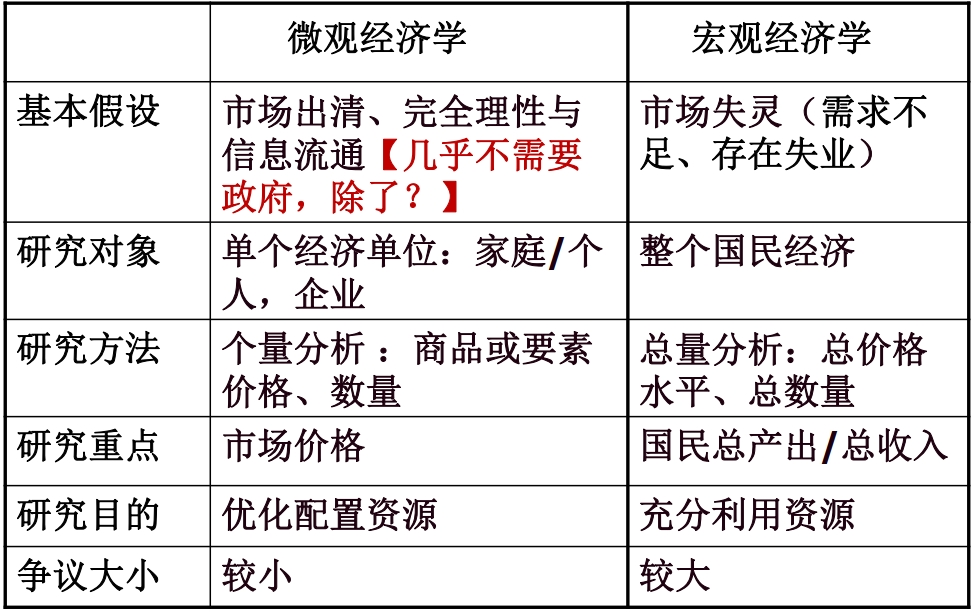
\includegraphics[width=0.5\textwidth]{微观经济学vs宏观经济学.png}
  \caption{微观经济学vs.宏观经济学}
\end{figure}

\subsection{一国收入(经济总量)的衡量}
\textcolor{red}{国内生产总值(Gross Domestic Product GDP)}: 在某一既定时期\textbf{一个国家内生产}的所有最终物品与劳务的市场价值。

什么不包括在GDP之内?e.g.家里生产和消费而没有进入市场的大多数商品和服务;非法生产和销售的项目,如毒品。
\begin{itemize}
  \item “…最终…”:GDP只包括最终物品的价值,而不包括中间品的价值(价值只能计算一次)
  \item “…物品与劳务…”:它既包括有形的物品,也包括无形的劳务
  \item “…生产的…”:它包括现期生产的物品与劳务,并不包括涉及过去生产的东西的交易
  \item “…一个国家之内的…”:它衡量的生产价值是在一个国家的地理范围之内
  \item “…在某一既定时期内…”:它衡量某一既定时期内进行的生产的价值,通常这个时期是一年和一个季度
\end{itemize}

其他收入衡量指标:
\begin{itemize}
  \item 国民收入总值 Gross National Product (GNP):是一国永久居民(称为国民)所赚到的总收入 
  \item 国民生产净值 Net National Product (NNP):是一国居民的总收入减去折旧的消耗; 折旧是经济中设备和建筑物存量的磨损或损耗
  \item 国民收入 National Income:是一国居民在物品与劳务生产中赚到的总收入
\end{itemize}

GDP的组成部分(支出法):包括了用于国内生产的物品和服务的所有支出形式:
\begin{itemize}
  \item Consumption (C) 消费(C)
  \item Investment (I) 投资(I)
  \item Government Purchases (G) 政府购买(G)
  \item Net Exports (NX) 净出口(NX)
\end{itemize}

GDP的组成部分:
\begin{itemize}
  \item 消费 (C):家庭除了购买\textbf{新住房}以外用于物品与劳务的支出
  \item 投资 (I) ≠ 金融当中的投资:指用于\textbf{资本设备、存货和建筑物}的支出,其中包括家庭用于购买新住房的支出。是对用于在未来生产物品与服务的物品的购买
\end{itemize}